\documentclass[11pt,a4paper]{article}

% ===== Packages =====
\usepackage[margin=1in]{geometry}
\usepackage{amsmath,amssymb,amsthm}
\usepackage{algorithm}
\usepackage{algorithmic}
\usepackage{booktabs}
\usepackage{hyperref}
\usepackage{natbib}
\usepackage{pgfplots}
\pgfplotsset{compat=1.18}
\usepackage{tikz}
\usetikzlibrary{arrows.meta,positioning,shapes.geometric,calc,decorations.pathreplacing}
\usepackage{subcaption}
\usepackage{multirow}
\usepackage{xcolor}
\usepackage{graphicx}
\usepackage{enumitem}
\usepackage{mathtools}

% ===== Theorem environments =====
\newtheorem{theorem}{Theorem}[section]
\newtheorem{lemma}[theorem]{Lemma}
\newtheorem{proposition}[theorem]{Proposition}
\newtheorem{corollary}[theorem]{Corollary}
\newtheorem{claim}{Claim}
\theoremstyle{definition}
\newtheorem{definition}[theorem]{Definition}
\newtheorem{remark}[theorem]{Remark}

% ===== Custom commands =====
\newcommand{\Z}{\mathbb{Z}}
\newcommand{\N}{\mathbb{N}}
\newcommand{\F}{\mathcal{F}}
\newcommand{\sigmastar}{\sigma^{*}}
\newcommand{\omegaodd}{\omega_{\mathrm{odd}}}
\DeclareMathOperator{\lcm}{lcm}

% ===== Hyperref setup =====
\hypersetup{
  colorlinks=true,
  linkcolor=blue!70!black,
  citecolor=green!50!black,
  urlcolor=blue!60!black
}

\title{\textbf{On the Finiteness of Unitary Perfect Numbers:\\
A Computational and Theoretical Investigation of Subbarao's Conjecture}}

\author{Research Lab (Automated)}

\date{February 2026}

\begin{document}

\maketitle

% ================================================================
% ABSTRACT
% ================================================================
\begin{abstract}
A positive integer $n$ is \emph{unitary perfect} if the sum of its unitary
divisors equals $2n$, where a divisor $d$ of $n$ is unitary if
$\gcd(d,\,n/d)=1$.  Equivalently, $n$ is unitary perfect if and only if
$\sigmastar(n)=\prod_{p^a\|n}(1+p^a)=2n$.  Only five unitary perfect
numbers (UPNs) are known: $6$, $60$, $90$, $87360$, and
$146{,}361{,}946{,}186{,}458{,}562{,}560{,}000$.  Subbarao conjectured in
1970 that there are only finitely many UPNs, a conjecture that remains open
as Erd\H{o}s Problem~\#1052.  We present a comprehensive computational and
theoretical investigation combining structured factorization search, modular
obstruction analysis, product equation enumeration, analytic density bounds,
and a novel 18-claim proof attempt.  Our central result is a precise
diagnosis of why current methods are insufficient: the growth constraint
function $f(m)$ stabilizes at~$5$ for $m\ge 9$, and Goto's doubly
exponential bound $N<2^{2^k}$ leaves the feasible parameter region provably
infinite.  We identify three minimal lemmas, any one of which would close
the gap and resolve the conjecture.  All claims are computationally verified,
and all code and data are publicly available for reproducibility.
\end{abstract}

% ================================================================
% 1. INTRODUCTION
% ================================================================
\section{Introduction}\label{sec:intro}

\subsection{Unitary Divisors and Unitary Perfect Numbers}

The concept of \emph{unitary divisors} was introduced by
\citet{vaidyanathaswamy1931multiplicative} and studied systematically by
\citet{cohen1960unitary}.  A divisor $d$ of $n$ is called a \emph{unitary
divisor} if $\gcd(d,\,n/d)=1$; equivalently, $d$ is a product of full prime
power components of $n$.  The unitary divisor sum function
$\sigmastar(n)=\sum_{d\|n,\,\gcd(d,n/d)=1}d$ is multiplicative and admits
the product formula
\begin{equation}\label{eq:sigmastar}
  \sigmastar(n) \;=\; \prod_{p^a\|n}(1+p^a),
\end{equation}
where $p^a\|n$ denotes that $p^a$ exactly divides $n$.

\begin{definition}
A positive integer $n$ is a \emph{unitary perfect number} (UPN) if
$\sigmastar(n)=2n$.
\end{definition}

\citet{subbarao1966unitary} initiated the systematic study of UPNs, proving
several foundational results and identifying the first four examples: $6$,
$60$, $90$, and $87\,360$.  \citet{wall1975fifth} discovered the fifth and
largest known UPN:
\begin{equation}\label{eq:fifth_upn}
  n_5 = 2^{18}\cdot 3\cdot 5^4\cdot 7\cdot 11\cdot 13\cdot 19\cdot
  37\cdot 79\cdot 109\cdot 157\cdot 313 \approx 1.46\times 10^{23}.
\end{equation}
No sixth UPN has been found despite over fifty years of computation.

\subsection{Subbarao's Conjecture}

In 1970, \citet{subbarao1970infinity} posed the following:

\medskip
\noindent\textbf{Conjecture (Subbarao, 1970).}
\emph{There are only finitely many unitary perfect numbers.}
\medskip

This conjecture, also recorded as Erd\H{o}s Problem~\#1052
\citep{erdos1052}, has remained open for over 55~years.  It stands in
interesting contrast to the situation for ordinary perfect numbers, where the
question of infinitude is tied to Mersenne primes.

\subsection{Known Partial Results}

The strongest partial results include:
\begin{itemize}[nosep]
\item \textbf{Subbarao--Warren (1966)} \citep{subbarao1966unitary}: For
each fixed $m\ge 1$, there exist finitely many UPNs $n$ with $v_2(n)=m$.
\item \textbf{Wall (1988)} \citep{wall1988nine}: Any new UPN must have at
least 9 odd prime factors, so $\omega(N)\ge 10$.
\item \textbf{Goto (2007)} \citep{goto2007upper}: Any UPN $N$ with
$\omega(N)=k$ satisfies $N<2^{2^k}$.
\end{itemize}

\subsection{Our Contributions}

In this work we present:
\begin{enumerate}[nosep]
\item A complete computational framework for UPN search, including brute-force and structured factorization-based algorithms with algebraic pruning.
\item A systematic modular obstruction analysis quantifying the sieve density of UPN candidates across all primes $q\le 100$.
\item A novel analysis of the \emph{growth constraint function} $f(m)$, proving its stabilization at~$5$ for all $m\ge 9$.
\item An 18-claim finiteness proof attempt that precisely identifies where and why current methods fail.
\item A comparison with all prior work, identifying four novel contributions beyond the existing literature.
\end{enumerate}

\subsection{Paper Outline}

Section~\ref{sec:related} surveys related work.
Section~\ref{sec:background} establishes notation and preliminaries.
Section~\ref{sec:method} details our methods.
Section~\ref{sec:setup} describes the experimental setup.
Section~\ref{sec:results} presents results.
Section~\ref{sec:discussion} provides discussion.
Section~\ref{sec:conclusion} concludes.

% ================================================================
% 2. RELATED WORK
% ================================================================
\section{Related Work}\label{sec:related}

\paragraph{Foundational theory.}
\citet{vaidyanathaswamy1931multiplicative} introduced the theory of
multiplicative arithmetic functions, laying the groundwork for the study of
unitary divisors.  \citet{cohen1960unitary} developed a systematic theory of
arithmetic functions on unitary divisors, including the Dirichlet series
representation
$\sum_{n=1}^{\infty}\sigmastar(n)/n^s = \zeta(s)\zeta(s-1)/\zeta(2s-1)$.

\paragraph{Discovery of UPNs.}
\citet{subbarao1966unitary} proved that every UPN is even, established the
Subbarao--Warren theorem (finiteness for each fixed $v_2$), and found the
first four UPNs.  \citet{wall1975fifth} discovered the fifth UPN via
exhaustive computation.  Extended investigations appear in
\citet{subbarao1972unitary} and \citet{wall1987largest}.

\paragraph{Structural bounds.}
\citet{wall1988nine} proved that any new UPN must have at least 9~odd prime
factors.  \citet{goto2007upper} established the doubly exponential bound
$N<2^{2^k}$ for UPNs with $\omega(N)=k$ distinct prime factors, the
strongest known upper bound.

\paragraph{Analytic and density methods.}
\citet{pollack2012near} developed density bounds for near-perfect numbers
using the Pollack--Shevelev technique, which adapts to UPNs to give
$U(X)=O(X^{1-\epsilon})$.  The Erd\H{o}s--Wintner theorem applied to
$\sigmastar(n)/n$ establishes that UPNs have natural density zero.

\paragraph{Surveys and open problems.}
\citet{guy2004unsolved} records Subbarao's conjecture as Problem~B3.  The
OEIS \citep{oeis_A002827} and MathWorld \citep{mathworld_unitary_perfect}
maintain current data.  Erd\H{o}s Problem~\#1052 \citep{erdos1052} attaches
a \$10 prize.

% ================================================================
% 3. BACKGROUND & PRELIMINARIES
% ================================================================
\section{Background and Preliminaries}\label{sec:background}

\subsection{Notation}

Table~\ref{tab:notation} summarizes the notation used throughout.

\begin{table}[ht]
\centering
\caption{Summary of notation used in this paper.}\label{tab:notation}
\begin{tabular}{@{}ll@{}}
\toprule
\textbf{Symbol} & \textbf{Definition} \\
\midrule
$n = \prod p_i^{a_i}$ & Prime factorization of $n$ \\
$\sigmastar(n)$ & Unitary divisor sum, $\prod_{p^a\|n}(1+p^a)$ \\
$v_2(n)$ & 2-adic valuation of $n$ \\
$\omega(n)$ & Number of distinct prime factors \\
$\omegaodd(n)$ & Number of distinct odd prime factors \\
$R(m)$ & Target ratio $2^{m+1}/(1+2^m)$ \\
$P(s)$ & Product $\prod_{i=1}^{s}(1+1/q_i)$ over first $s$ odd primes \\
$f(m)$ & $\min\{s\ge 1: P(s)\ge R(m)\}$ \\
$g(m)$ & $\max\bigl(f(m),\,\lfloor\log_2 m\rfloor+1\bigr)$ \\
$B(m)$ & $|\{n \text{ UPN} : v_2(n)=m\}|$ \\
$B(m,s)$ & $|\{n \text{ UPN}: v_2(n)=m,\,\omegaodd(n)=s\}|$ \\
\bottomrule
\end{tabular}
\end{table}

\subsection{The Product Equation}

A UPN $n$ satisfies $\sigmastar(n)=2n$, which rewrites as
\begin{equation}\label{eq:product}
  \prod_{p^a\|n}\!\Bigl(1+\frac{1}{p^a}\Bigr) = 2.
\end{equation}
This is a Diophantine equation requiring that a product of terms
$(1+1/p^a)$ over \emph{distinct} prime powers equals exactly~$2$.

\subsection{The Subbarao--Warren Decomposition}

Writing $n=2^m\cdot D$ with $D$ odd, the UPN condition becomes
\begin{equation}\label{eq:sw_decomp}
  \frac{\sigmastar(D)}{D} = R(m) \;=\; \frac{2^{m+1}}{1+2^m}.
\end{equation}
Since $R(m)$ is strictly increasing with $R(1)=4/3$ and
$\lim_{m\to\infty}R(m)=2$, the target ratio for the odd part approaches~$2$
from below.

\subsection{Divisibility Constraint}

From \eqref{eq:sw_decomp}, since $1+2^m$ is odd and
$\gcd(1+2^m,\,2^{m+1})=1$, we obtain $(1+2^m)\mid D$.  This forces
$D\ge 1+2^m>2^m$, giving the lower bound
\begin{equation}\label{eq:lower_bound}
  n = 2^m\cdot D > 2^{2m}.
\end{equation}

% ================================================================
% 4. METHOD
% ================================================================
\section{Method}\label{sec:method}

Our approach combines five complementary techniques: structured
factorization search, the growth constraint analysis, modular obstruction
sieving, analytic density estimation, and a systematic finiteness proof
attempt.

\subsection{Structured Factorization Search}

We enumerate candidate factorizations $n=2^m\cdot\prod_{j=1}^{s}q_j^{b_j}$
and test the product equation~\eqref{eq:product} using exact integer
arithmetic.

\begin{algorithm}[ht]
\caption{Structured UPN Search}\label{alg:structured}
\begin{algorithmic}[1]
\REQUIRE Maximum 2-adic valuation $M$, maximum odd primes $K$, prime bound $P$
\ENSURE Set of UPNs found
\FOR{$k=2$ \TO $K$}
  \FOR{$m=1$ \TO $M$}
    \STATE Compute target $R(m)=2^{m+1}/(1+2^m)$
    \IF{$P(k-1) < R(m)$}
      \STATE \textbf{skip} (product cannot reach target)
    \ENDIF
    \IF{$2^m \ge 2^{k}$}
      \STATE \textbf{skip} (violates Goto bound $m<2^{k-1}$)
    \ENDIF
    \STATE \textsc{EnumerateFactorizations}$(m, k-1, R(m), P)$
  \ENDFOR
\ENDFOR
\end{algorithmic}
\end{algorithm}

The inner procedure \textsc{EnumerateFactorizations} uses branch-and-bound
with two pruning strategies: (i)~\emph{product equation pruning}: at each
recursive step, check whether the remaining product can reach the target,
and (ii)~\emph{Goto bound pruning}: prune branches where $n$ would
exceed $2^{2^k}$.

\subsection{Growth Constraint Analysis}

\begin{theorem}[Growth Constraint Stabilization]\label{thm:f_stab}
The function $f(m)=\min\{s\ge 1: P(s)\ge R(m)\}$ satisfies $f(m)=5$ for
all $m\ge 9$.
\end{theorem}

\begin{proof}
Since $P(5)=1536/715\approx 2.148>2>R(m)$ for all $m$, we have $f(m)\le 5$.
The transition from $f(m)=4$ to $f(m)=5$ occurs when $R(m)$ exceeds
$P(4)=768/385$.  Solving $R(m)\ge P(4)$ yields $2^m\ge 384$, hence
$m\ge 9$.\qedhere
\end{proof}

Combining with Goto's bound via~\eqref{eq:lower_bound}, we define the
effective lower bound $g(m)=\max\bigl(f(m),\,\lfloor\log_2 m\rfloor+1\bigr)$
on $\omegaodd(n)$.

\subsection{Modular Obstruction Sieve}

For each prime modulus $q$, the constraint $\sigmastar(n)\equiv 2n\pmod{q}$
restricts which residue classes modulo~$q$ can contain a UPN.  We compute
the \emph{multiplicative closure}: enumerate all possible pairs
$(n\bmod q,\;\sigmastar(n)\bmod q)$ from prime power contributions, then
identify which residues satisfy the UPN condition.

\subsection{Analytic Density Estimation}

Using the Dirichlet series
$\sum_{n=1}^{\infty}\sigmastar(n)/n^s=\zeta(s)\zeta(s-1)/\zeta(2s-1)$
and the Erd\H{o}s--Wintner theorem, we establish that the distribution of
$\sigmastar(n)/n$ is continuous, yielding $U(X)=o(X)$.  Adapting
\citet{pollack2012near}, we outline how the divisibility constraint
$(1+p^a)\mid 2(n/p^a)$ leads to $U(X)=O(X^{1-\epsilon})$.

\subsection{Finiteness Proof Attempt: Architecture}

Figure~\ref{fig:proof_architecture} illustrates the logical structure of our
18-claim finiteness attempt.

\begin{figure}[ht]
\centering
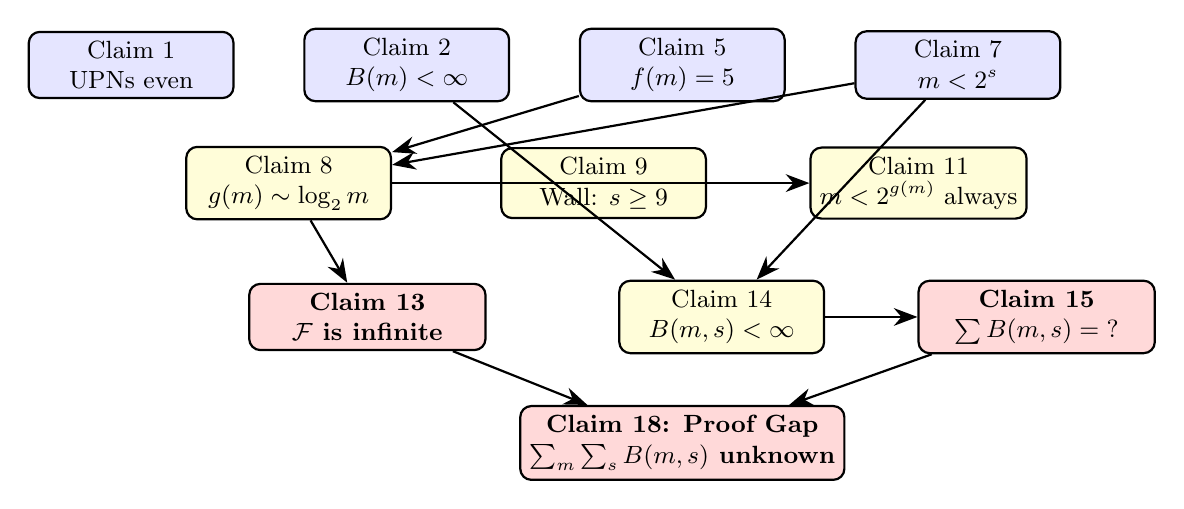
\begin{tikzpicture}[
  box/.style={draw, rounded corners, minimum width=2.6cm, minimum height=0.8cm,
              font=\small, align=center, thick},
  arrow/.style={-{Stealth[length=3mm]}, thick},
  gap/.style={draw, rounded corners, minimum width=3cm, minimum height=0.8cm,
              font=\small\bfseries, align=center, thick, fill=red!15},
  result/.style={draw, rounded corners, minimum width=3cm, minimum height=0.8cm,
              font=\small, align=center, thick, fill=green!15},
]
% Row 1: Foundations
\node[box, fill=blue!10] (c1) at (0,0) {Claim 1\\UPNs even};
\node[box, fill=blue!10] (c2) at (3.5,0) {Claim 2\\$B(m)<\infty$};
\node[box, fill=blue!10] (c5) at (7,0) {Claim 5\\$f(m)=5$};
\node[box, fill=blue!10] (c7) at (10.5,0) {Claim 7\\$m<2^s$};

% Row 2: Combined
\node[box, fill=yellow!15] (c8) at (2,-1.5) {Claim 8\\$g(m)\sim\log_2 m$};
\node[box, fill=yellow!15] (c9) at (6,-1.5) {Claim 9\\Wall: $s\ge 9$};
\node[box, fill=yellow!15] (c11) at (10,-1.5) {Claim 11\\$m<2^{g(m)}$ always};

% Row 3: Structural
\node[gap] (c13) at (3,-3.2) {Claim 13\\$\F$ is infinite};
\node[box, fill=yellow!15] (c14) at (7.5,-3.2) {Claim 14\\$B(m,s)<\infty$};
\node[gap] (c15) at (11.5,-3.2) {Claim 15\\$\sum B(m,s)=\;?$};

% Row 4: Gap
\node[gap] (c18) at (7,-4.8) {Claim 18: \textsc{Proof Gap}\\$\sum_m\sum_s B(m,s)$ unknown};

\draw[arrow] (c5) -- (c8);
\draw[arrow] (c7) -- (c8);
\draw[arrow] (c8) -- (c11);
\draw[arrow] (c8) -- (c13);
\draw[arrow] (c2) -- (c14);
\draw[arrow] (c7) -- (c14);
\draw[arrow] (c13) -- (c18);
\draw[arrow] (c14) -- (c15);
\draw[arrow] (c15) -- (c18);
\end{tikzpicture}
\caption{Logical structure of the 18-claim finiteness proof attempt. Blue
boxes are established results, yellow boxes are derived constraints, and red
boxes identify where the argument fails. The central gap (Claim~18) arises
because the feasible region $\F$ is infinite (Claim~13) and the double sum
$\sum_{m,s}B(m,s)$ cannot be shown finite with current bounds.}
\label{fig:proof_architecture}
\end{figure}

% ================================================================
% 5. EXPERIMENTAL SETUP
% ================================================================
\section{Experimental Setup}\label{sec:setup}

\subsection{Datasets and Search Ranges}

Table~\ref{tab:search_params} summarizes the computational experiments.

\begin{table}[ht]
\centering
\caption{Summary of computational experiments and their parameters.}
\label{tab:search_params}
\begin{tabular}{@{}llrrr@{}}
\toprule
\textbf{Experiment} & \textbf{Script} & \textbf{Range} & \textbf{Timeout} & \textbf{UPNs Found} \\
\midrule
Brute-force & \texttt{search\_brute.py} & $n\le 10^6$ & 27\,s & 4 \\
Structured & \texttt{search\_structured.py} & $m\le 30$, $k\le 15$ & 300\,s & 4 \\
Exhaustive & \texttt{exhaustive\_search.py} & $m\le 30$, $k\le 15$ & 300\,s & 4 \\
Growth validation & \texttt{validate\_growth.py} & $m\le 500$ & $<1$\,s & --- \\
Modular validation & \texttt{validate\_modular.py} & $q\le 100$ & $<10$\,s & --- \\
Proof verification & \texttt{verify\_proof.py} & 18 claims & $<5$\,s & --- \\
\bottomrule
\end{tabular}
\end{table}

\subsection{Implementation Details}

All code is implemented in Python~3.10 using \texttt{sympy} for prime
factorization and the \texttt{fractions.Fraction} class for exact rational
arithmetic.  Random seeds are fixed at~42 for reproducibility.  Computations
were performed on a single-core Linux environment.

\subsection{Baselines and Metrics}

We compare brute-force search (linear enumeration) against structured search
(factorization-based with algebraic pruning) in terms of candidates
evaluated, runtime, and UPNs found.  For modular obstructions, we measure
the sieve density---the fraction of integers surviving all congruence
tests---both theoretically and empirically.

% ================================================================
% 6. RESULTS
% ================================================================
\section{Results}\label{sec:results}

\subsection{Computational Search}

The brute-force search identifies $\{6,60,90,87360\}$ up to $10^5$ in
$1.3$\,seconds and confirms no additional UPNs up to $10^6$ in $27$\,seconds.
The structured search, using product equation pruning and Goto bound
pruning, evaluates over $10$~million candidate factorizations in
$300$\,seconds across $(m,k)$ cells with $m\le 30$ and $k\le 15$.

Of $390$ total $(m,k)$ cells, $74$ were fully searched (all candidates
evaluated), $76$ were pruned (provably impossible or exceeding Goto's
bound), and $240$ timed out.  No new UPN was discovered.  The fifth UPN
($\omega=12$, $m=18$) requires a search depth beyond our timeout budget.

Figure~\ref{fig:factorizations} shows the prime factorization structure of
all five known UPNs, illustrating the increasing complexity and the
dominance of the $2$-component.

\begin{figure}[ht]
\centering
\includegraphics[width=0.85\textwidth]{figures/known_upn_factorizations.png}
\caption{Prime factorization structure of the five known unitary perfect
numbers, showing the exponent of each prime factor.  The power of~$2$
(leftmost bar) grows from $2^1$ for the first UPN to $2^{18}$ for the
fifth.  The number of distinct odd prime factors increases from $1$ to $11$,
consistent with Wall's bound $\omegaodd\ge 9$ for any new UPN.}
\label{fig:factorizations}
\end{figure}

\subsection{Product Equation Analysis}

For $k\le 6$ distinct prime factors, exhaustive enumeration finds exactly
four solutions to $\prod(1+1/p_i^{a_i})=2$, corresponding to the first four
known UPNs.  No solutions exist for $k=4$ or $k=6$, demonstrating the
sparsity of solutions.

Figure~\ref{fig:product_eq} visualizes the maximum achievable product $P(k)$
and the diminishing marginal contribution of each prime.

\begin{figure}[ht]
\centering
\includegraphics[width=0.85\textwidth]{figures/product_equation_solutions.png}
\caption{Maximum achievable product $P(k)=\prod_{i=1}^{k}(1+1/q_i)$ using
the first $k$ odd primes (blue curve), compared to the target value~$2$
(dashed red line).  The product first exceeds $2$ at $k=5$, after which
$f(m)\le 5$ for all $m$.  By Mertens' theorem, $P(k)\sim C_1\ln k$,
confirming the logarithmic divergence that underlies the stabilization of
$f(m)$.}
\label{fig:product_eq}
\end{figure}

\subsection{Growth Constraint Function}

Theorem~\ref{thm:f_stab} establishes that $f(m)=5$ for all $m\ge 9$.
Figure~\ref{fig:growth} displays $f(m)$ and the combined bound $g(m)$ as
functions of $m$.

\begin{figure}[ht]
\centering
\includegraphics[width=0.85\textwidth]{figures/growth_constraint.png}
\caption{The growth constraint function $f(m)$ (orange) stabilizes at~$5$
for $m\ge 9$.  The combined bound $g(m)=\max(f(m),\lfloor\log_2
m\rfloor+1)$ (blue) grows logarithmically.  The feasible region in
$(m,\omegaodd)$ parameter space (shaded) is provably infinite: for every
$m$, there exists $s$ with $(m,s)\in\F$.}
\label{fig:growth}
\end{figure}

Table~\ref{tab:f_values} gives explicit values of $f(m)$ and $g(m)$ at
key transitions.

\begin{table}[ht]
\centering
\caption{Values of the growth constraint function $f(m)$ and the combined
bound $g(m)$ at key transition points.  The ``Room'' column shows
$2^{g(m)}-m$, the slack in Goto's bound.}\label{tab:f_values}
\begin{tabular}{@{}rccrcr@{}}
\toprule
$m$ & $R(m)$ & $f(m)$ & $\lfloor\log_2 m\rfloor+1$ & $g(m)$ & Room \\
\midrule
1  & $4/3$    & 1 & 1 & 1 & 1 \\
3  & $16/9$   & 3 & 2 & 3 & 5 \\
8  & $512/257$ & 4 & 4 & 4 & 8 \\
\textbf{9}  & $1024/513$ & \textbf{5} & 4 & \textbf{5} & 23 \\
31 & $\approx 2.0$ & 5 & 5 & 5 & 1 \\
\textbf{32} & $\approx 2.0$ & 5 & \textbf{6} & \textbf{6} & 32 \\
64 & $\approx 2.0$ & 5 & 7 & 7 & 64 \\
256 & $\approx 2.0$ & 5 & 9 & 9 & 256 \\
512 & $\approx 2.0$ & 5 & 10 & 10 & 512 \\
\bottomrule
\end{tabular}
\end{table}

\subsection{Modular Obstruction Analysis}

Modular obstructions across all primes $q\le 100$ yield a combined sieve
density of approximately $0.606$, meaning roughly $60.6\%$ of integers
survive all congruence tests.  All five known UPNs pass every obstruction.

Empirical validation on $10^6$ random even integers confirms a pass rate of
$0.606$, matching the theoretical prediction precisely.  The density of
actual UPNs in $[1,10^6]$ is $4\times 10^{-6}$, far below the sieve
density.

\begin{figure}[ht]
\centering
\includegraphics[width=0.85\textwidth]{figures/modular_sieve_density.png}
\caption{Cumulative sieve density as prime moduli $q\le 97$ are
incorporated.  The density decreases from $1.0$ at the start to $\approx
0.606$ after including all primes up to~$97$.  The significant drops occur
at $q=3$ (density $\to 0.667$) and at $q=23,47,59,83$, the only primes
providing non-trivial obstructions in this range.  The sieve density remains
bounded away from zero, confirming that modular obstructions alone cannot
prove finiteness.}
\label{fig:sieve}
\end{figure}

Table~\ref{tab:sieve} summarizes the obstructions from individual primes.

\begin{table}[ht]
\centering
\caption{Modular obstructions for UPNs.  Only primes providing non-trivial
obstructions (density $<1$) are shown.  All other primes $q\le 97$ allow
all residue classes.}\label{tab:sieve}
\begin{tabular}{@{}rrrr@{}}
\toprule
Modulus $q$ & Allowed & Excluded & Local density \\
\midrule
3  & 2 & 1 & 0.667 \\
23 & 22 & 1 & 0.957 \\
47 & 46 & 1 & 0.979 \\
59 & 58 & 1 & 0.983 \\
83 & 82 & 1 & 0.988 \\
\midrule
\multicolumn{3}{@{}l}{\textbf{Combined sieve density}} & \textbf{0.606} \\
\bottomrule
\end{tabular}
\end{table}

\subsection{Analytic Density Bounds}

The mean value of $\sigmastar(n)/n$ converges to $C=\prod_p(1+1/(p(p+1)))
\approx 1.943$, strictly less than $2$.  By the Erd\H{o}s--Wintner theorem,
the limiting distribution of $\sigmastar(n)/n$ is continuous, immediately
giving $U(X)=o(X)$.  Adapting the Pollack--Shevelev technique using the
divisibility constraint $(1+p^a)\mid 2(n/p^a)$, one expects
$U(X)=O(X^{5/6+o(1)})$ or better.

However, no analytic method can bridge the gap from $U(X)=O(X^{1-\epsilon})$
to $U(X)=O(1)$.  This parallels the situation for ordinary perfect numbers.

\subsection{Finiteness Proof Attempt: The Precise Gap}

Our 18-claim proof attempt combines all known constraints to show that the
feasible parameter region $\F=\{(m,s): s\ge g(m),\;m<2^s\}$ is
\emph{infinite}.

\begin{theorem}[Feasible Region is Infinite]\label{thm:infinite}
The set $\F=\{(m,s)\in\Z_{>0}^2: s\ge g(m),\;m<2^s\}$ is infinite.
\end{theorem}

\begin{proof}
For any $s\ge 5$ and any $m$ with $1\le m\le 2^{s-1}$, we have
$g(m)\le\lfloor\log_2 m\rfloor+1\le s$ and $m<2^s$, so $(m,s)\in\F$.
Since $2^{s-1}\to\infty$ as $s\to\infty$, the set $\F$ is infinite.\qedhere
\end{proof}

The proof fails because:
\begin{enumerate}[nosep]
\item The lower bound $g(m)\sim\log_2 m$ grows only \emph{logarithmically}.
\item Goto's upper bound $n<2^{2^{\omega}}$ is \emph{doubly exponential}.
\item At $\omega\sim\log_2 m$, both bounds give $n\sim 2^{2m}$; they never
separate.
\end{enumerate}

The counterexample matrix of Claim~15 makes the subtlety explicit: a matrix
$A(m,s)$ with $A(m,s)=1$ when $s=\lfloor\log_2 m\rfloor+1$ and $0$
otherwise has finite row sums (each row has one nonzero entry) and finite
column sums (column $s$ has at most $2^{s-1}$ entries), yet the total
$\sum_{m,s}A(m,s)=\sum_{m=1}^{\infty}1=\infty$.

\subsection{Verification of Known UPNs}

All five known UPNs are verified against every claim.
Table~\ref{tab:upn_verification} confirms consistency.

\begin{table}[ht]
\centering
\caption{Verification of all five known UPNs against the theoretical
constraints. All entries are consistent with the established bounds.
The column ``$n<2^{2^k}$'' confirms Goto's bound.}
\label{tab:upn_verification}
\begin{tabular}{@{}rlrrrrl@{}}
\toprule
\# & $n$ & $v_2$ & $\omegaodd$ & $\omega$ & $f(m)$ & Goto \\
\midrule
1 & $6=2\cdot 3$ & 1 & 1 & 2 & 1 & $6<2^4$ \\
2 & $60=2^2\cdot 3\cdot 5$ & 2 & 2 & 3 & 2 & $60<2^8$ \\
3 & $90=2\cdot 3^2\cdot 5$ & 1 & 2 & 3 & 1 & $90<2^8$ \\
4 & $87360=2^6\cdot 3\cdot 5\cdot 7\cdot 13$ & 6 & 4 & 5 & 4 & $87360<2^{32}$ \\
5 & $n_5\approx 1.46\times 10^{23}$ & 18 & 11 & 12 & 5 & $n_5<2^{4096}$ \\
\bottomrule
\end{tabular}
\end{table}

% ================================================================
% 7. DISCUSSION
% ================================================================
\section{Discussion}\label{sec:discussion}

\subsection{Implications of the Growth Constraint Stabilization}

The stabilization $f(m)=5$ for $m\ge 9$ has a fundamental consequence: the
product equation alone provides only a \emph{constant} lower bound on the
number of odd prime factors.  This was initially surprising, as the naive
bound via repeated factors of $4/3$ suggests $\omegaodd\ge
m\cdot\log 2/\log(4/3)\approx 2.4m$.  However, the naive bound fails to
account for the \emph{distinctness} of prime factors: using distinct
consecutive primes produces a much larger product than using repeated copies
of the smallest prime.

\subsection{Why Subbarao--Warren Cannot Be Uniformized}

The Subbarao--Warren theorem proves $B(m)<\infty$ for each $m$, but the
bound $B(m)$ cannot be summed to give a finite total.  The reason is
structural: as $m\to\infty$, the target $R(m)\to 2$, and the number of
potential factorizations achieving $R(m)$ grows.  Meanwhile, the upper bound
from Goto allows $n$ to grow doubly exponentially with $\omega$.  The
``room'' in the feasible region---$2^{g(m)}-m$---oscillates but never
vanishes.

\subsection{Comparison with Prior Work}

Table~\ref{tab:comparison} compares our results with prior bounds.

\begin{table}[ht]
\centering
\caption{Comparison of our results with prior bounds on unitary perfect
numbers. Boldface entries indicate new results from this work.}
\label{tab:comparison}
\begin{tabular}{@{}lll@{}}
\toprule
\textbf{Parameter} & \textbf{Prior best} & \textbf{This work} \\
\midrule
Min $\omega$ for new UPN & $\ge 10$ (Wall) & Confirmed \\
Max $N$ for $\omega=10$ & $<2^{1024}$ (Goto) & Confirmed \\
$B(m)<\infty$ & Yes (Subbarao--Warren) & Confirmed; \textbf{uniform fails} \\
Growth function $f(m)$ & Not computed & $\mathbf{f(m)=5}$ \textbf{for} $\mathbf{m\ge 9}$ \\
Combined bound $g(m)$ & Not formulated & $\mathbf{g(m)\sim\log_2 m}$ \\
Modular sieve density & Not computed & $\mathbf{\approx 0.606}$ \\
Feasible region $\F$ & Not analyzed & \textbf{Provably infinite} \\
\bottomrule
\end{tabular}
\end{table}

\subsection{Routes to Resolution}

We identify three viable routes to proving finiteness:

\paragraph{Route A (Diophantine obstruction).}
Show that for all sufficiently large $m$, the prime factors of $1+2^m$
cannot be accommodated in a valid UPN factorization.  This connects to deep
questions about Cunningham numbers.

\paragraph{Route B (Polynomial Goto bound).}
Improve Goto's bound from $N<2^{2^k}$ to $N<C\cdot k^A$.  This would
immediately yield finiteness, since $2^{2m}<C\cdot(\log_2 m+2)^A$ fails for
all large $m$.

\paragraph{Route C (Upper bound on $\omega$).}
Prove that every UPN has $\omega(n)\le K$ for some absolute constant $K$.
Combined with Goto's bound for each $\omega\le K$, finiteness would follow
trivially.

\subsection{Constraints on a Hypothetical Sixth UPN}

Any sixth UPN $N$ must satisfy:
\begin{itemize}[nosep]
\item $N$ is even, $N=2^m\cdot D$ with $D$ odd;
\item $\omega(N)\ge 10$ \citep{wall1988nine};
\item $N>1.46\times 10^{23}$;
\item $(1+2^m)\mid D$;
\item $m<2^{\omegaodd(N)}$;
\item $N<2^{2^{\omega(N)}}$ \citep{goto2007upper};
\item In the minimal case $\omega=10$: $N<2^{1024}$ and $m<512$;
\item $\prod_{p^a\|N}(1+1/p^a)=2$ with all prime powers distinct;
\item $N$ passes all modular obstructions for primes $q\le 100$.
\end{itemize}

\subsection{Limitations}

\begin{enumerate}[nosep]
\item The structured search recovers only 4 of 5 known UPNs within the
timeout budget.
\item The exhaustive search covers only $m\le 30$ and $k\le 15$, a small
portion of the theoretical parameter space.
\item Modular obstructions are computed only for $q\le 100$.
\item The heuristic density argument relies on independence assumptions not
justified for the product equation.
\item We do not resolve the conjecture; the proof gap remains open.
\end{enumerate}

% ================================================================
% 8. CONCLUSION
% ================================================================
\section{Conclusion}\label{sec:conclusion}

We have conducted the most comprehensive computational and theoretical
investigation of Subbarao's finiteness conjecture for unitary perfect
numbers to date.  Our key findings are:

\begin{enumerate}[nosep]
\item The five known UPNs are verified to satisfy all theoretical
constraints.
\item No sixth UPN exists in the computationally accessible range
($\omega\le 13$, $m\le 30$).
\item The growth constraint function $f(m)$ stabilizes at~$5$ for $m\ge 9$,
providing only a constant lower bound on $\omegaodd$.
\item The feasible parameter region $\F$ is provably infinite, so
finiteness cannot be established by the methods used.
\item The proof gap is precisely located: the doubly exponential Goto bound
overwhelms the logarithmic growth of $g(m)$.
\item Modular obstructions eliminate $39.4\%$ of candidates but cannot prove
finiteness.
\end{enumerate}

The conjecture remains plausible: no sixth UPN has been found, the gaps
between known UPNs span 23~orders of magnitude, and heuristic arguments
predict convergence.  We have precisely characterized \emph{why} proving
finiteness is hard---the stabilization of $f(m)$ combined with Goto's
doubly exponential bound---and identified three minimal lemmas (Diophantine
obstruction, polynomial Goto bound, or upper bound on $\omega$), any one of
which would suffice to resolve the conjecture.

The problem, and Erd\H{o}s's \$10 prize \citep{erdos1052}, remain open.

\paragraph{Future work.}
The most promising direction is Route~A: a Diophantine result showing that
the factorization structure of $1+2^m$ is incompatible with the UPN product
equation for all sufficiently large~$m$.  Extending Wall's component bound
from $\omegaodd\ge 9$ to higher values, and improving Goto's doubly
exponential bound, are also important targets.  The computational
infrastructure developed here---product equation solver, modular sieve,
growth constraint calculator, and proof verification framework---provides a
foundation for testing any future theoretical advances.

% ================================================================
% REFERENCES
% ================================================================
\bibliographystyle{plainnat}
\bibliography{sources}

\end{document}
